\setcounter{section}{8}

\Needspace{5\baselineskip}
\hypertarget{delta-attention}{%
\section{Delta Attention}\label{delta-attention}}

\Needspace{5\baselineskip}
\hypertarget{i.-background-2}{%
\subsection{I. Background}\label{i.-background-2}}

Earlier, we noted that when a Transformer is viewed as dynamic gradient descent, the most central role of Softmax is the ``induction head'': even in a long context, it ensures that attention remains focused on the x matching y, rather than becoming ``diffuse.'' Linear attention is already sufficient for functions such as updating ``weights W'' by gradient descent according to the difference between actual and predicted values. Given linear attention's lower GPU-memory consumption, Kimi Delta Attention (KDA) proposes a hybrid architecture: it mixes linear-attention layers and full-Softmax-attention layers at a 3:1 ratio. Most layers use linear attention to efficiently handle local semantic aggregation, state transfer, and continual feature updates (memory writing), while a few Softmax layers (which store a complete KV cache) perform high-precision global information retrieval, routing across extremely long distances, and complex pattern matching.

\Needspace{5\baselineskip}
\hypertarget{ii.-from-linear-attention-to-deltanet}{%
\subsection{II. From Linear Attention to DeltaNet}\label{ii.-from-linear-attention-to-deltanet}}

\Needspace{5\baselineskip}
Traditional linear attention is expressed as:

\[
S_t=S_{t-1}+k_tv_t^\top
\]

This explicit matrix (hidden state) \(S\) lies on the residual branch. Its objective is to fit the relationship between \(K\) and \(V\), taking \(Q\) as input and outputting context-aggregated \(V\) (which is added to the original input as a residual, rather than already incorporating the residual internally and directly outputting the overall result \(y\), as \(W\) does). For layer \(l\), the relationship between input \(x_t^{(l)}\) and output \(x_t^{(l+1)}\) (the input to layer \(l+1\)) is:

\[
\mathrm{Output}_t^{(l)}=\left(S_t^{(l)}\right)^\top q_t^{(l)}
\]

\[
x_t^{(l+1)}=x_t^{(l)}+\mathrm{Output}_t^{(l)}
\]

Earlier, we noted that the Transformer as a whole (including the residual stream) is equivalent to implicitly maintaining a weight matrix \(W\) satisfying \(y=Wx\). During in-context learning, \(S_t^\top q_t\) on the residual branch effectively plays the role of \(\Delta W x_t\): based on the relationship between \(K_i\) (\(x_i\)) and \(V_i\) (\(Wx_i-y_i\)) in the available data, it determines the gap between the true \(y_t\) and \(Wx_t\).

\Needspace{5\baselineskip}
However, this model has serious problems during training. The update formula for \(S\) is equivalent to using a correlation loss to learn the mapping from \(k_t\) to \(v_t\):

\[
\mathcal{L}_{\mathrm{Linear}}=-\left\langle S^\top k_t,v_t\right\rangle
\]

The resulting gradient gives the update formula for \(S\) above. Notice that this update is unbounded: even if \(S\) has already learned the mapping from \(k_t\) to \(v_t\), for every token (the \(t\)th token), whenever \(k_t\) and \(v_t\) arrive, it calculates a nonzero gradient \(-k_tv_t^\top\) and blindly adds it to \(S\). This may cause the matrix elements to grow without bound and produce severe information interference when processing long contexts (because the dimension is finite, the additions cannot always be orthogonal).

\Needspace{5\baselineskip}
With Softmax, because attention scores sum to 1, the output vector is constrained to the convex hull of the existing tokens' value vectors. There is no such constraint here, so we modify the loss function for each time \(t\):

\[
\mathcal{L}_{\mathrm{Delta}}=\frac{1}{2}\left\lVert S^\top k_t-v_t\right\rVert^2
\]

\Needspace{5\baselineskip}
Run one gradient descent step with adaptive learning rate \(\beta_t\):

\[
S_t=S_{t-1}+\beta_tk_t\left(v_t-k_t^\top S_{t-1}\right)
\]

Note that, unlike the matrix \(W\) discussed earlier, which performs gradient descent at each time \(t\) using \((x_1,y_1),\ldots,(x_t,y_t)\) (while also seeking to prevent \(y_t\) from producing a gradient), this uses only \((k_t,v_t)\) for gradient descent. The fundamental reason for this difference is the different optimization objectives:

In the theoretical paper (standard attention), the model faces an external few-shot in-context-learning task.

\begin{itemize}
\tightlist
\item
  The prompt you give the model resembles an examination paper: given \((x_1,y_1),(x_2,y_2),\ldots,(x_n,y_n)\), find the \(y_{\mathrm{test}}\) corresponding to \(x_{\mathrm{test}}\).
\end{itemize}

In KDA (a linear RNN), the model faces its own internal memory-compression task of autoregressive state tracking.

\begin{itemize}
\tightlist
\item
  KDA has no knowledge of the few-shot examination question you are working on. Its sole mission is to replace the KV cache by compressing the continuously arriving historical text into a fixed-size matrix \(S\).
\item
  In autoregressive generation, time moves only forward. When the model reads token \(t\), the features \(k_t\) and \(v_t\) produced by this token are ``known facts.''
\item
  KDA must immediately use this known fact to update \(S_{t-1}\to S_t\), so that when token \(t+1\), or even token \(t+100\), arrives with a query, the memory contains a record of token \(t\).
\end{itemize}

The KDA paper (and DeltaNet) explicitly identifies this as online gradient descent.

\begin{itemize}
\tightlist
\item
  Batch gradient descent is also the method we normally use to train large models. It requires calculating the losses for an entire batch of data (all tokens), averaging them, and then updating the weights once. Its objective is to find a global optimum.
\item
  Online gradient descent is the flexible, feature-dependent strategy used by KDA's internal \(S\) matrix. During autoregressive generation, tokens stream in one at a time; the model cannot retrieve the entire history of previous tokens and recalculate every error just to calculate the update at step \(t\).
\item
  Therefore, it considers only the current token \(t\), calculates an instantaneous gradient \(\nabla_S\mathcal{L}_t(S_{t-1})\), and immediately takes a small step (of size \(\beta_t\)) to update the memory.
\end{itemize}

\Needspace{5\baselineskip}
At the same time, KDA avoids ``catastrophic forgetting'' as much as possible:

\begin{itemize}
\tightlist
\item
  When token \(t\) arrives, the memory matrix \(S_{t-1}\) it encounters is not a blank slate. \(S_{t-1}\) is the accumulated result of the preceding \(t-1\) online gradient descent steps.
\item
  When KDA calculates the error and subtracts \(\beta_t k_t k_t^\top S_{t-1}\), it does not completely overturn \(S_{t-1}\). Because \(\beta_t\) is usually a scalar between \(0\) and \(1\), less than \(1\) (dynamically predicted by the model), it only fine-tunes and refines the vast historical memory \(S_{t-1}\) along the specific feature direction (\(k_t\)) of token \(t\).
\end{itemize}

\Needspace{5\baselineskip}
\hypertarget{iii.-kimi-delta-attention}{%
\subsection{III. Kimi Delta Attention}\label{iii.-kimi-delta-attention}}

\Needspace{5\baselineskip}
When new data arrive at time t, the hidden state S is updated as:

\[
S_t=\left(I-\beta_t k_t k_t^\top\right)\mathrm{Diag}(\alpha_t)S_{t-1}+\beta_t k_t v_t^\top
\]

Here, \(\mathrm{Diag}(\alpha_t)\) is a diagonal matrix that left-multiplies \(S_{t-1}\), assigning a forget-gate-like mechanism to the parameters in each row. This has some similarity to Adam's per-parameter adaptive learning rates.

\Needspace{5\baselineskip}
Kimi defines the relevant matrices as:

\[
\begin{aligned}
q_t^{(l)},k_t^{(l)}
&=\mathrm{L2Norm}\left(\mathrm{Swish}\left(\mathrm{ShortConv}\left(W_q^{(l)}x_t^{(l)}\right)\right)\right)\in\mathbb{R}^{d_k},\\
v_t^{(l)}
&=\mathrm{Swish}\left(\mathrm{ShortConv}\left(W_v^{(l)}x_t^{(l)}\right)\right)\in\mathbb{R}^{d_v},\\
\alpha_t^{(l)}
&=f\left(W_\alpha^{(l)}x_t^{(l)}\right)\in[0,1]^{d_k},\\
\beta_t^{(l)}
&=\mathrm{Sigmoid}\left(W_\beta^{(l)}x_t^{(l)}\right)\in[0,1].
\end{aligned}
\]

Of course, engineering implementations could also try approaches in which \(\alpha_t\) or \(\beta_t\) is jointly determined by \(x_t\) and \(\alpha_{t-1}\) or \(\beta_{t-1}\) (potentially helping to judge a token's value within a long sequence more accurately).

\Needspace{5\baselineskip}
Overall architecture:

\begin{figure}[htbp]
\centering
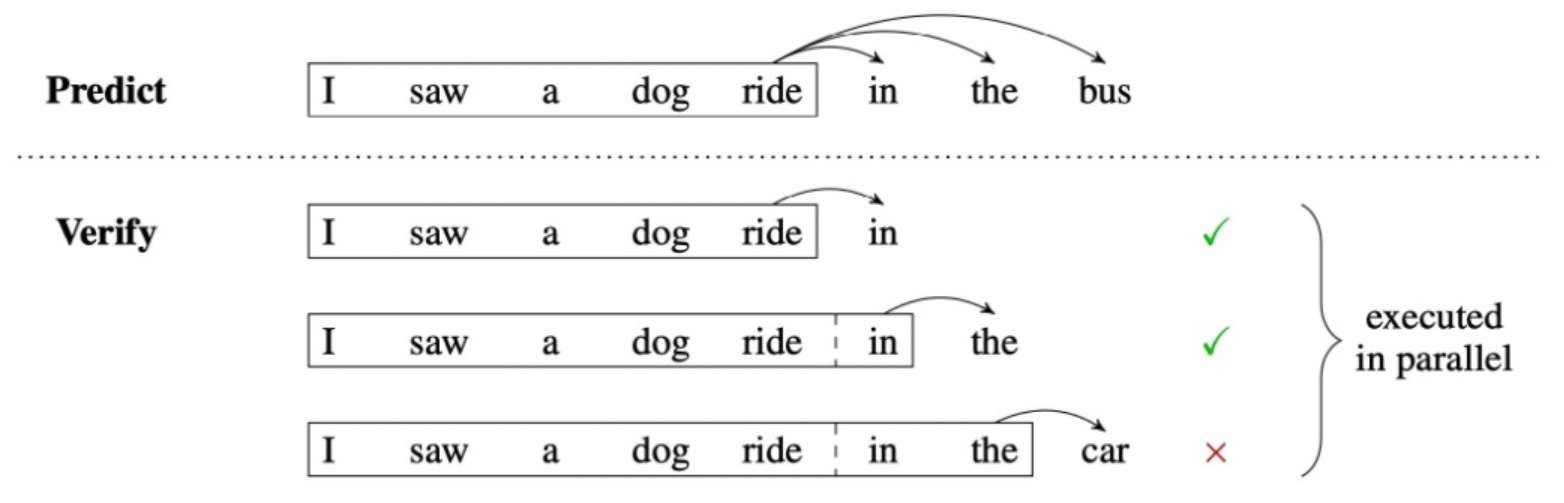
\includegraphics{images/image-0024.png}
\caption{Diagram of the Kimi Delta Attention hybrid architecture}
\end{figure}

\Needspace{5\baselineskip}
\hypertarget{iv.-kda-and-rnns}{%
\subsection{IV. KDA and RNNs}\label{iv.-kda-and-rnns}}

In principle, KDA is essentially an RNN. Why, then, does KDA work better than traditional RNN architectures such as LSTM?

\begin{enumerate}
\def\labelenumi{\arabic{enumi}.}
\item
  Hidden-state capacity: LSTM has a d-dimensional hidden-state vector, whereas KDA has a d*d-dimensional hidden-state matrix.
\item
  Whether large-scale parallel training on GPUs is possible
\end{enumerate}

\Needspace{5\baselineskip}
During model training, when processing a long text containing thousands or tens of thousands of tokens:

\begin{itemize}
\tightlist
\item
  LSTM is locked into serial computation. Its state update formula is \(h_t=\tanh(Wx_t+Uh_{t-1})\); notice the nonlinear activation function \(\tanh\). This means that step \(t-1\) must finish completely and yield the exact \(h_{t-1}\) before step \(t\) can begin. On a GPU with thousands or tens of thousands of streaming processors, LSTM must still calculate one step after another, leaving much of the GPU's computational power idle.
\item
\Needspace{5\baselineskip}
  KDA has a parallelizable linear recurrence. Ignoring the specific coefficients, KDA's structural formula can be written as:
\end{itemize}

\[
S_t=A_tS_{t-1}+V_t
\]

\Needspace{5\baselineskip}
This formula is completely linear in the hidden state \(S\) (with no \(\tanh\) or Sigmoid in the way). By the associativity of matrix multiplication, we can expand the time sequence:

\[
S_3=A_3(A_2S_1+V_2)+V_3=(A_3A_2)S_1+A_3V_2+V_3
\]

\Needspace{5\baselineskip}
Specifically, for the two stages of inference:

A. Feedback integration stage (prefill mode): supports parallelism across tokens

When the environment returns a new piece of text (such as search results or a change in environment state), KDA does not need to update its state serially one token at a time as an RNN does.

\begin{itemize}
\tightlist
\item
  Chunkwise-parallel algorithm: KDA uses the associativity of linear attention. Mathematical transformations convert its recurrence into a chunkwise-parallel form.
\item
  Implementation: if the environment returns \(L\) tokens, KDA can treat these \(L\) tokens as one ``chunk'' and use GPU Tensor Cores for highly parallel matrix operations. A single pass processes all \(L\) tokens and directly obtains the final state \(S_{t+L}\).
\item
  Comparison: when traditional models process new feedback, the computational complexity of the KV cache grows quadratically with total length, whereas KDA's complexity for processing new feedback is linear in total length.
\end{itemize}

B. Text generation stage (decoding mode): generation in a single pass, without parallelism across tokens

\Needspace{5\baselineskip}
When the model begins generating a new response action based on feedback:

\begin{itemize}
\tightlist
\item
  Single pass: generating each new token indeed requires only one forward pass of \(O(1)\) complexity. It only needs to read the previous state \(S_{t-1}\) and calculate \(S_t\), without rescanning the entire preceding context.
\item
  Parallelism limitation: because generation is autoregressive, token \(N+1\) must depend on the state after token \(N\) is generated. Parallelism across tokens is therefore impossible during generation (unless combined with techniques such as speculative sampling).
\end{itemize}

Of course, if the sequence returned by the environment is long, we often process it in chunks of a certain number of tokens to suit the GPU.

In any case, KDA can use operators such as FlashAttention for acceleration.

\begin{enumerate}
\def\labelenumi{\arabic{enumi}.}
\setcounter{enumi}{2}
\tightlist
\item
  Mathematical nature: LSTM updates are ``heuristic.'' The forget and input gates inside LSTM are formulas devised by earlier researchers through intuition and experimentation. The network only implicitly learns a ``threshold'' for deciding what to retain and discard; it is essentially a feature filter.
\end{enumerate}

KDA updates follow ``first principles.'' As in our preceding derivation, the KDA update formula is strictly equivalent to online gradient descent, that is, training an internal linear regression model online.

Faced with new data, KDA calculates the prediction error and precisely modifies the memory matrix \(S_t\) in the opposite direction to the gradient. This rigorous mathematical foundation gives KDA a performance ceiling far above traditional RNNs for complex logical reasoning and in-context learning.

\Needspace{5\baselineskip}
\hypertarget{v.-kda-and-meta-learning}{%
\subsection{V. KDA and Meta-Learning}\label{v.-kda-and-meta-learning}}

We can regard KDA as a meta-learning architecture. In standard Transformers, this meta-learning is implicit; KDA makes it explicit.

\Needspace{4\baselineskip}
\begin{enumerate}
\def\labelenumi{\arabic{enumi}.}
\tightlist
\item
  Outer loop: learn ``how to learn in context''
\end{enumerate}

During pretraining, we use standard optimizers (such as AdamW) on thousands or tens of thousands of GPUs to update KDA's physical parameters using massive corpora: the projection weights \(W_Q,W_K,W_V\) that generate \(q,k,v\), and the forgetting gates \(\alpha,\beta\).

\Needspace{5\baselineskip}
These physical parameters are the ``meta-parameters.'' AdamW does not teach the model specific knowledge; it teaches the model:

\begin{itemize}
\tightlist
\item
  What learning rate \(\beta\) to assign when encountering different kinds of data.
\item
  What features should activate the forget gate \(\alpha\).
\item
  How to extract \(k\) and \(v\) from text in a way most suitable for calculating residuals.
\end{itemize}

\Needspace{4\baselineskip}
\begin{enumerate}
\def\labelenumi{\arabic{enumi}.}
\setcounter{enumi}{1}
\tightlist
\item
  Inner loop: online gradient descent
\end{enumerate}

After the model is deployed, you give it a long prompt. At this point, the physical parameters (meta-parameters) are frozen, and the AdamW optimizer is no longer active.

\Needspace{5\baselineskip}
However, KDA's internal memory matrix \(S_t\) is activated. As your input data flow in step by step, KDA strictly follows the delta rule taught by the outer loop, that is, the online gradient descent formula:

\[
S_t=S_{t-1}+\beta_tk_t\left(v_t-k_t^\top S_{t-1}\right)
\]

When the token at time \(t\) enters the KDA layer, the hidden state is updated by gradient descent based on \(k_t\) and \(v_t\), changing from \(S_{t-1}\) to \(S_t\) and incorporating the new information at time \(t\). At the same time, it has already retained information from the first \(t-1\) tokens through the preceding \(t-1\) gradient descent steps (stored as a prior in \(S_{t-1}\)). Passing \(q_t\) through \(S_t\), rich in information from \(t\) contextual tokens, enables new tasks to be completed through in-context learning.

\Needspace{4\baselineskip}
\begin{enumerate}
\def\labelenumi{\arabic{enumi}.}
\setcounter{enumi}{2}
\tightlist
\item
  Other parameters (such as the embedding layer and input projection): learn prior knowledge
\end{enumerate}

During pretraining, the model's internal embedding layer and input projection (MLP layer) memorize various kinds of prior knowledge about the human world, such as ``In what year did Qin Shi Huang become emperor?'' This prior knowledge is compressed into these model parameters, forming an enormous high-dimensional feature subspace that ensures inputs are mapped to vectors consistent with their actual meanings before entering the attention layers. For example, when ``apple'' is input, the MLP instantly maps it into a feature coordinate system containing countless meanings such as ``fruit, red, technology company, Newton.''

In addition, for an input token, the model uses its prior parameters to judge whether to activate the in-context learning mechanism. For a simple general-knowledge question (such as ``What is the capital of France?''), the model does not need complex in-context gradient descent: its MLP (prior knowledge) can directly output the features of ``Paris.'' In this case, \(W_0\ne 0\), while \(\Delta W\to 0\) in subsequent attention layers. For distributions the model has not seen during training, it lets \(W_0\to 0\) (almost no prior, to avoid interfering with in-context learning) and leaves the analysis to the subsequent \(\Delta W\).

\FloatBarrier
\Needspace{5\baselineskip}
\hypertarget{references-99}{%
\subsection{References}\label{references-99}}

\vspace{0.25em}
\begin{itemize}
\tightlist
\item
  Kimi Team. (2025). \href{https://arxiv.org/abs/2510.26692}{Kimi Linear: An Expressive, Efficient Attention Architecture}. arXiv:2510.26692.
\end{itemize}

\clearpage
